% ============================ PHASE 1 ==================================
\newpage
\setcounter{section}{0}
\phase{Phase one \textbullet\ The molecule}{Hydrogen, from the ground up}{What it is, where it already hides in an ordinary Indian day, and the truth about hydrogen trains and cars.}

\subsection{The lightest thing there is, and why that is awkward}

Hydrogen is the simplest atom in the universe: one proton, one electron. On Earth it almost never sits around on its own. It is locked inside water (H\textsubscript{2}O) and inside fossil fuels such as natural gas (CH\textsubscript{4}). So the first thing to understand is the one most headlines skip: \textbf{hydrogen is not an energy source. It is an energy carrier.} Someone has to spend energy to pull it out of water or gas, and the whole argument about ``green'' versus ``grey'' is really an argument about \emph{where that energy comes from}.

The second thing is its odd personality. By weight it is a champion: a kilogram of hydrogen carries about 120 megajoules, nearly three times the 44 MJ in a kilogram of petrol. By volume it is a featherweight: even chilled into a liquid, a litre holds about 8 MJ against petrol's 32 MJ. To make it fit anywhere useful you either squeeze it to 350–700 times atmospheric pressure or cool it to $-252.8$\,°C \cite{doe}. \confH

\begin{center}
\begin{tikzpicture}[x=1mm,y=1mm,font=\small]
  \node[anchor=west,font=\eyebrowfont\fontsize{6.6}{8}\selectfont,text=brass] at (0,30) {ENERGY PER KILOGRAM (MJ)};
  \fill[sblue,rounded corners=1pt] (0,21) rectangle (120*0.45,26); \node[anchor=west] at (120*0.45+2,23.5) {Hydrogen \ 120};
  \fill[ink2!55,rounded corners=1pt] (0,14) rectangle (44*0.45,19); \node[anchor=west] at (44*0.45+2,16.5) {Petrol \ 44};
  \node[anchor=west,font=\eyebrowfont\fontsize{6.6}{8}\selectfont,text=brass] at (90,30) {ENERGY PER LITRE, LIQUID (MJ)};
  \fill[sblue,rounded corners=1pt] (90,21) rectangle (90+8*1.4,26); \node[anchor=west] at (90+8*1.4+2,23.5) {Hydrogen \ 8};
  \fill[ink2!55,rounded corners=1pt] (90,14) rectangle (90+32*1.4,19); \node[anchor=west] at (90+32*1.4+2,16.5) {Petrol \ 32};
  \node[anchor=west,text width=150mm,font=\small\itshape,text=ink2] at (0,7) {Light to carry, bulky to store. That one fact explains why hydrogen suits big, fixed industrial plants far better than small moving vehicles. Source: \cite{doe}.};
\end{tikzpicture}
\end{center}

\subsection{Where hydrogen already touches your day}

Most people think hydrogen is a fuel of the future. It is mostly a chemical of the present. The world used almost 100 million tonnes of it in 2024 \cite{ieanews2025}, and in India it shows up in four places you would not expect.

\begin{center}
\begin{tikzpicture}[
  card/.style={rounded corners=2pt,fill=wash,draw=none,minimum height=50mm,text width=32mm,align=left,inner sep=6pt,anchor=north west},
  big/.style={font=\display\fontsize{18}{20}\selectfont,text=ink},
  lab/.style={font=\eyebrowfont\fontsize{6.6}{8}\selectfont,text=brass}]
\foreach \ii/\ttl/\num/\desc/\col in {
 0/FOOD/48\%/{of humanity was fed by fertiliser nitrogen from hydrogen-based ammonia by 2008 \cite{erisman2008}. About 70\% of all ammonia goes into fertiliser \cite{ieaammonia2021}.}/sgreen,
 1/FUEL/2.6 Mt/{of hydrogen a year goes into Indian refineries, mainly to strip sulphur out of petrol and diesel \cite{igef2021}.}/sblue,
 2/FAT/Vanaspati/{is vegetable oil hardened by adding hydrogen, the cheaper cousin of ghee \cite{foodnav2012}.}/sochre,
 3/MATERIALS/Methanol/{made from hydrogen feeds paints, resins and plastics; chlor-alkali, glass and electronics plants use it too \cite{igef2021}.}/sviolet}{
  \node[card] (c\ii) at (\ii*38mm,0) {\textcolor{\col}{\rule{8mm}{1.6pt}}\\[4pt]{\eyebrowfont\fontsize{6.6}{8}\selectfont\color{brass}\ttl}\\[3pt]{\display\fontsize{17}{19}\selectfont\color{ink}\num}\\[3pt]{\footnotesize\desc}};
}
\end{tikzpicture}
\end{center}

The scale is the surprise. India used roughly 5.6 million tonnes of hydrogen made at home in 2018–19, plus about 1.1 million tonnes hidden inside the ammonia and methanol it imported, for a total near 6.7 million tonnes \cite{igef2021}. Nearly all of it is grey. Analysts expect demand to roughly double to about 12 million tonnes by 2030, with fertiliser and refining still taking the lion's share \cite{tribune2025}. \confM\ (the base figures were modelled from chemistry rather than measured, and they are now seven years old.)

\begin{figure}[H]
\centering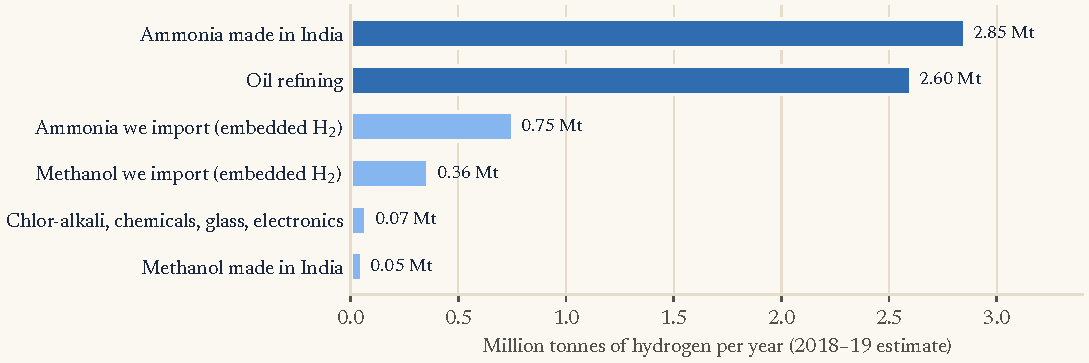
\includegraphics[width=0.98\textwidth]{figures/india_h2_use.pdf}
\caption{India's hydrogen, by where it ends up. Two uses (fertiliser ammonia and refining) account for over 80\%. Data: \cite{igef2021}.}
\end{figure}

\begin{plainwords}
If you ate a roti today, rode a bike on petrol, or bought biscuits made with vanaspati, you used hydrogen. You just never saw it, because it was made and consumed inside a factory fence. That is why the cleanest, quickest win is not a new hydrogen gadget but \emph{changing how the hydrogen we already use gets made}.
\end{plainwords}

\subsection{The hot topic: trains, cars and the hydrogen dream}

\subsubsection{What actually happened in Haryana.}
On 17 July 2026 the Prime Minister flagged off India's first hydrogen passenger train at Jind \cite{bt2026}. The facts are impressive. It is a 10-coach set carrying about 2,600 passengers over the 89 km between Jind and Sonipat. Two power cars of 1,200 kW each run on proton-exchange-membrane fuel cells, with a design speed of 110 km/h. The hydrogen is made on site at Jind by electrolysis, compressed to 500 bar, dispensed at 350 bar, and a store holds nearly 3,000 kg \cite{skh2train2026}. Officials call it the largest-capacity hydrogen train in service anywhere \cite{bt2026}. \confH

\subsubsection{What it proves, and what it does not.}
It proves Indian engineers can design, build and certify a hydrogen system end to end, including PESO safety approval \cite{skh2train2026}. That matters. What it does not prove is that hydrogen is the future of Indian rail. By November 2025, \textbf{99.2\% of Indian Railways' broad-gauge network was already electrified} \cite{indinfra2025}. An electric train on an overhead wire uses the electricity directly; a hydrogen train turns electricity into hydrogen, then hydrogen back into electricity, and loses a lot on the way. So the hydrogen train's natural home is the last fraction of track: heritage and hill lines where wires are impractical, which is exactly where Indian Railways says it will deploy the technology \cite{skh2train2026}. \confH

Germany ran this experiment first, and the lesson is sobering. Lower Saxony, home of the world's first hydrogen passenger trains, decided in 2023 that battery trains were cheaper and would replace the rest of its diesel fleet with them \cite{railtech2023}. One analyst reports that by August 2025 only four of its fourteen hydrogen trainsets were running, for lack of replacement fuel-cell modules \cite{barnard2026}. \confM\ (opinion piece, but the 2023 battery decision is well documented.)

\subsubsection{And hydrogen cars?}
Here the physics is unkind. Volkswagen's own engineers put it plainly: of the renewable electricity you start with, a battery car delivers about 70–80\% to the wheels; a hydrogen fuel-cell car delivers about 25–35\% \cite{vw2020}. The market has voted accordingly.

\begin{center}
\begin{tikzpicture}[x=1mm,y=1mm]
\begin{scope}
\node[anchor=west,font=\eyebrowfont\fontsize{6.6}{8}\selectfont,text=brass] at (0,40) {OUT OF 100 UNITS OF CLEAN ELECTRICITY};
\fill[faint,rounded corners=1pt] (0,28) rectangle (70,34); \fill[sgreen,rounded corners=1pt] (0,28) rectangle (75*0.7,34);
\node[anchor=west,font=\small] at (72,31) {\textbf{70–80} reach the wheels of a battery car};
\fill[faint,rounded corners=1pt] (0,18) rectangle (70,24); \fill[sred,rounded corners=1pt] (0,18) rectangle (30*0.7,24);
\node[anchor=west,font=\small] at (72,21) {\textbf{25–35} reach the wheels of a hydrogen car};
\node[anchor=west,font=\footnotesize\itshape,text=ink2] at (0,12) {Source: \cite{vw2020}. Bars drawn at the range midpoints.};
\end{scope}
\begin{scope}[shift={(0,-30)}]
\foreach \x/\bg/\sm/\src in {0/{17 million+}/{electric cars sold worldwide in 2024}/ieagevo2025, 52/{$\approx$12,900}/{hydrogen fuel-cell vehicles sold in 2024 (16,011 in 2025)}/asiae2026, 104/{1 : 1,300}/{roughly one hydrogen car for every 1,300 electric cars}/asiae2026}{
\fill[wash,rounded corners=2pt] (\x,0) rectangle (\x+48,26);
\node[anchor=north west,font=\display\fontsize{16}{18}\selectfont,text=ink] at (\x+3,23) {\bg};
\node[anchor=north west,text width=42mm,font=\footnotesize] at (\x+3,13) {\sm\ \cite{\src}};
}
\end{scope}
\end{tikzpicture}
\end{center}

The 2024 fuel-cell figure is back-calculated from SNE Research's 2025 total of 16,011 units and its 24.4\% growth rate \cite{asiae2026}; the ratio uses IEA's 17 million electric cars \cite{ieagevo2025}. \confH\ on direction, \confM\ on the exact ratio.

Michael Liebreich's widely used ``hydrogen ladder'' reaches the same verdict from the other end. Its top row, labelled ``no alternative'', holds the jobs hydrogen already does, mostly fertiliser and refining. Its bottom row, which he calls ``the row of doom'', holds passenger cars, bulk e-fuels and power generation from hydrogen that was never stored \cite{liebreich2023}. \confH

\begin{figure}[H]
\centering
\begin{tikzpicture}[
  rung/.style={rounded corners=1.5pt,minimum height=8.2mm,text width=#1,align=left,inner sep=4pt,font=\footnotesize},
  lbl/.style={font=\eyebrowfont\fontsize{6.2}{7}\selectfont,text=brass,anchor=east}]
\def\W{116mm}
\node[rung=\W,fill=sgreen!22] (a) at (0,0) {\textbf{Fertiliser ammonia, oil refining, methanol and chemicals.} Hydrogen is a raw material here, not a fuel. Nothing else does the chemistry.};
\node[rung=\W,fill=sgreen!12,below=1.3mm of a] (b) {\textbf{Green steel (direct reduction), ship fuels made from hydrogen (ammonia, methanol).} Few alternatives at scale.};
\node[rung=\W,fill=wash,below=1.3mm of b] (c) {\textbf{Long-haul heavy trucks, non-electrified rail, seasonal energy storage.} Possible, contested, geography-dependent.};
\node[rung=\W,fill=sred!8,below=1.3mm of c] (d) {\textbf{City buses, two-wheelers, home cooking and heating.} Batteries, heat pumps and induction usually win.};
\node[rung=\W,fill=sred!18,below=1.3mm of d] (e) {\textbf{Passenger cars, burning hydrogen in ordinary power plants.} The ``row of doom''.};
\node[lbl] at ([xshift=-3mm]a.west) {NO ALTERNATIVE};
\node[lbl] at ([xshift=-3mm]b.west) {STRONG CASE};
\node[lbl] at ([xshift=-3mm]c.west) {NICHE};
\node[lbl] at ([xshift=-3mm]d.west) {WEAK};
\node[lbl] at ([xshift=-3mm]e.west) {ROW OF DOOM};
\draw[-{Stealth[length=3mm]},line width=1pt,ink2] ([xshift=4mm]e.south east) -- ([xshift=4mm]a.north east) node[midway,right,font=\footnotesize\itshape,text=ink2,align=left] {value of\\ using\\ hydrogen};
\end{tikzpicture}
\caption{My five-rung reading of where hydrogen earns its keep. Top and bottom rows match Liebreich's ladder v5.0 \cite{liebreich2023}; the middle rows are my own grouping.}
\end{figure}

\begin{verdict}[My verdict on the dream]
The vision of ``hydrogen engines replacing petrol engines and EVs'' is the wrong dream for India. For cars, scooters and city buses, batteries win on physics, and the market is already settled. The \emph{right} dream is bigger and less visible: make the six-odd million tonnes of hydrogen India already uses clean, then use clean hydrogen for the jobs electricity cannot do (steel, ships, fertiliser). That is where it cuts emissions and imported gas at the same time. \confH
\end{verdict}

\subsection{Is our project connected to the train and the car?}

Yes, more than it looks. The Jind refuelling station is a miniature of exactly what we would build: electrolysers, compressors and storage tanks next to a source of power. Our plant would be the same idea at roughly a thousand times the scale.

A quick sense of size, using my base-case model (Section 3): a 100 MW alkaline plant running about 5,000 hours a year at 53 kWh per kilogram would make about \textbf{9,400 tonnes of hydrogen a year, or 26 tonnes a day}. Turned into ammonia, that is about \textbf{53,000 tonnes a year}, almost exactly the size of one mid-sized SECI green-ammonia contract \cite{seci2025}. The same 26 tonnes a day could refuel about 200 German-style hydrogen trains, each needing about 130 kg \cite{barnard2026}. \confM

\begin{figure}[H]
\centering
\begin{tikzpicture}[
  plant/.style={circle,fill=ink,text=paper,minimum size=24mm,align=center,font=\small\bfseries},
  use/.style={rounded corners=2pt,fill=wash,text width=40mm,align=left,inner sep=5pt,font=\footnotesize},
  flow/.style={-{Stealth[length=3mm]},color=#1}]
\node[plant] (p) at (0,0) {Our 100 MW\\ plant\\[1pt]{\normalfont\footnotesize 26 t H\textsubscript{2}/day}};
\node[use,anchor=west] (f) at (3.4,1.9) {\textbf{Green ammonia for fertiliser.} 10-year SECI contracts exist today. \emph{Main gate.}};
\node[use,anchor=west] (r) at (3.4,0.15) {\textbf{Hydrogen for refineries.} 25-year contracts at ₹279–397/kg exist today \cite{jmkiocl2025,rwnrl2026}.};
\node[use,anchor=west] (s) at (3.4,-1.6) {\textbf{Steel and ship fuels.} The 2030s market. Real, but not yet contracted.};
\node[use,anchor=east] (m) at (-3.4,0.9) {\textbf{Mobility.} A small refuelling skid for trucks, buses or a train. \emph{Side door.}};
\node[use,anchor=east] (o) at (-3.4,-1.2) {\textbf{Oxygen by-product.} About 8 kg per kg of hydrogen, sellable to hospitals and industry.};
\draw[flow=sgreen,line width=4pt] (p) -- (f.west);
\draw[flow=sblue,line width=3pt] (p) -- (r.west);
\draw[flow=ink2,line width=1.6pt] (p) -- (s.west);
\draw[flow=sochre,line width=0.9pt] (p) -- (m.east);
\draw[flow=sviolet,line width=0.9pt] (p) -- (o.east);
\end{tikzpicture}
\caption{Where our hydrogen could go. Arrow thickness shows my ranking of near-term value, not exact volumes. The oxygen ratio follows from the chemistry of splitting water (8 kg O\textsubscript{2} per kg H\textsubscript{2}).}
\end{figure}

\begin{plainwords}[So can we help fuel the hydrogen train or a hydrogen bus?]
Technically, yes. A compressor and a dispenser bolted onto our plant would do it. Commercially, it should be a side door, not the main gate. A single train or bus fleet would use a fraction of one percent of our output, and its demand is uncertain. The customer who can sign a long contract for most of our output is a fertiliser company or a refinery. We build for them, and keep the mobility skid as a cheap option.
\end{plainwords}
